\chapter{Введение в робастное оценивание}

Схема, предложенная Мартином-Йохаи (Martin, Yohai, 1986), имеет вид:
$$y_t = u_t + z_t^{\gamma} \xi_t, \; t = \ton n$$
\begin{itemize}
 	\item[$\bullet$] здесь $\{u_t\}$ - <<полезный сигнал>> (временной ряд)
 	\item[$\bullet$] $\{z_t^{\gamma}\}$ - н.о.р.с.в., $z_1^{\gamma} \sim Bin (1, \gamma)$ с $0 \le \gamma \le 1$, $\gamma$ - уровень засорения
 	\item[$\bullet$] $\xi_t$ - н.о.р.с.в. - грубые выбросы, $\xi_1$ имеет распределение $\mu_{\xi} \in M_{\xi}$, распределение $\mu_{\xi}$ неизвестно, а множество $M_{\xi}$ известно
 	\item[$\bullet$] последовательности $\{u_t\}, \{z_t^{\gamma}\}, \{\xi_t\}$ независимы между собой
 \end{itemize} 

 Пусть $y_1, \dots, y_n$ - наблюдения, и распределение вектора $Y_n = (y_1, \dots, y_n)$ зависит от неизвестного параметра $\beta$. Пусть $\hat{\beta_n}$ - некоторая оценка $\beta$.\\

 \textbf{Основное предположение}\\
При любом $0 \le \gamma \le 1$ существует предел $\hat{\beta_n} \xrightarrow[n \to \infty]{P}\theta_{\gamma}, \; \theta_0 = \beta$, т.е. $\hat{\beta_n}$ состоятельна.

\begin{definition}\label{lec:8/def:1}
	Если существует предел
	$$IF (\theta_{\gamma}, \mu_{\xi}) := \underset{\gamma \to +0}{\overset{}{\lim}} \frac{\theta_{\gamma} - \theta_0}{\gamma}$$
	то $IF(\theta_{\gamma}, \mu_{\xi})$ называется \red{функционалом влияния} (influence function) оценки $\hat{\beta_n}$.
\end{definition}

Если функционал влияния существует, то
$$\theta_{\gamma} = \theta_0 + IF (\theta_{\gamma}, \mu_{\xi}) \gamma + \overline{o}(\gamma), \; \gamma \to +0$$
т.е. $IF (\theta_{\gamma}, \mu_{\xi})$ характеризует главный линейный по $\gamma$ член в разложении по $\gamma$ асимптотического смещения $\theta_{\gamma} - \theta_0 = \theta_{\gamma} - \beta$.

\begin{definition}\label{lec:8/def:2}
	Величина $CES (\theta_{\gamma}, M_{\xi}) := \underset{\mu_{\xi} \in M_{\xi}}{\sup} |IF (\theta_{\gamma}, \mu_{\xi})|$ (cross error sensivity) называется \red{чувствительностью} оценки $\hat{\beta_n}$ к засорениям (выбросам).
\end{definition}

Если $CES (\theta_{\gamma}, M_{\xi}) < \infty$, то главный член по $\gamma$ асимптотического смещения $IF (\theta_{\gamma}, \mu_{\xi})\gamma$ равномерно мал при малых $\gamma$.

\begin{definition}\label{lec:8/def:3}
	Если $CES (\theta_{\gamma}, M_{\xi}) < \infty$, то оценка $\hat{\beta_n}$ называется \red{робастной} по смещению, или \red{B-робастной}.
\end{definition}

\section{Пример о выборочном среднем}\label{lec:8/sec:4}

$$\begin{cases}
	u_t = a + \varepsilon_t, \; \varepsilon_t \text{ - ошибки измерений} \\
	y_t = u_t + z_t^{\gamma} \xi_t, \; t = \ton n, \;\; E |\xi_1| < \infty
\end{cases}$$
$\{\varepsilon_t\}$ - н.о.р.с.в., $E \varepsilon_1 = 0 \; \Rightarrow \; E u_t = a$.

Возьмем оценкой $a$ эмпирическое среднее $\overline{y} = n^{-1}\underset{t=1}{\overset{n}{\sum}}y_t$ - о.н.к. ($\underset{t=1}{\overset{n}{\sum}}(y_t - \theta)^2 \to \underset{\theta}{min}$), тогда:
$$\begin{gathered}
	\overline{y} \xrightarrow[]{P}E(u_1 + z_1^{\gamma} \xi_1) \\
	\text{(по теореме Колмогорова)}\\
	E(u_1 + z_1^{\gamma} \xi_1) = a + \gamma E \xi_1 = \theta_{\gamma}^{LS}
\end{gathered}$$
Функция $\theta_{\gamma}^{LS}$ (least square) определена при всех $\gamma$.
$$\frac{\partial \theta_{\gamma}^{LS}}{\partial \gamma} = E \xi_1 = IF (\theta_{\gamma}, \mu_{\xi})$$
Если $M_1$ - класс распределений с конечным первым моментом, то
$$CES (\theta_{\gamma}^{LS}, M_1) = \underset{\mu_{\xi}\in M_1}{sup} |E{\xi_1}| = \infty$$
т.е. $\overline{y}$ - не B-робастна на классе $M_1$. 

\section{Пример о выборочной медиане}\label{lec:9/sec:1}
Пусть 
$$u_t = a + \varepsilon_t, \; t = \ton n \eqno(1)$$ где $\{\varepsilon_t\}$ - н.о.р.с.в., $\varepsilon_t \sim G(x)$ и ф.р. $G(x)$ неизвестна, $G(0) = \frac{1}{2}$. Тогда ф.р. $u_t$ есть $F(x) = G(x-a)$, т.е. $F(a) = \frac{1}{2}$. Итак, ноль - медиана $G(x)$, а $a$ - медиана $F(x)$.\\

Если $\varepsilon_t$ имеет симметричное относительно нуля распределение (т.е. $\varepsilon_t \Ddef -\varepsilon_t$, что для непрерывной $G(x)$ равносильно условию $G(x) + G(-x) = 1$ при всех $x$), то условия выше выполняются автоматически.

Т.о. при сформулированных условиях оценку медианы можно использовать как оценку математического ожидания.\\

Пусть $u_{(1)} \le u_{(2)} \le \dots \le u_{(n)}$ будет вариационный ряд наблюдений $u_1, \dots, u_n$.

\begin{definition}\label{lec:9/def:1}
	Величина $\hat{m_n} = \begin{cases}
		u_{(k+1)}, \; n = 2 k - 1 \\
		\frac{u_{(k+1)} + u_{(k)}}{2}, \; n = 2 k
	\end{cases}, k = 1, 2, \dots$ называется \red{выборочной медианой} наблюдений $u_1, \dots, u_n$.
\end{definition}

Мы знаем, что если $G(x)$ дифференцируема в нуле, и $g(0) = G' (0) > 0$, то для выборочной медианы справедлива асимптотическая нормальность:
$$n^{\frac{1}{2}} (\hat{m_n} - a) \xrightarrow[n \to \infty]{d} N \left(0, \frac{1}{4 g^2 (0)}\right)$$
Если в (1) $\{\varepsilon_t\}$ - н.о.р., $E \varepsilon_t = 0, \; 0 < E \varepsilon_t^2 = \sigma^2 < \infty$, то $n^{\frac{1}{2}} (\overline{u} - a) \xrightarrow[n \to \infty]{d} N(0, \sigma^2)$. Значит АОЭ выборочной медианы относительно $\overline{u}$ равна $e_{\hat{m_n}, \overline{X}} = 4 g^2 (0) \sigma^2$.\\

Изучим B-робастность выборочной медианы. Пусть:
$$\begin{gathered}
	\begin{cases}
		u_t = a + \varepsilon_t \\
		y_t = u_t + z_t^{\gamma} \xi_t, \; t = \ton n
	\end{cases} \\
	\hat{m}_n^y = \begin{cases}
		y_{(k+1)}, n = 2k-1 \\
		\frac{y_{(k)} + y_{(k+1)}}{2}, n = 2k
	\end{cases}
\end{gathered}$$

\begin{theorem}[]\label{lec:9/the:1}
	Пусть существует производная $g(x) = G' (x)$, $g(x)$ непрерывна и ограничена, $g(0) > 0$, $G(0) = \frac{1}{2}$. Тогда:
	\begin{itemize}
		\item[1)] $\hat{m}_n^y \xrightarrow[n \to \infty]{P}\theta_{\gamma}^m$, $\theta_0 = a$
		\item[2)] существует функционал влияния выборочной медианы
		$$IF (\theta_{\gamma}^m, \mu_{\xi}) = \frac{1 - 2 E G(-\xi_1)}{2 g(0)}$$
		\item[3)] чувствительность выборочной медианы на классе всех возможных распределений $M_{\xi}$
		$$GES (\theta_{\gamma}^m, M_{\xi}) = \underset{\mu_{\xi} \in M_{\xi}}{\sup}|IF (\theta_{\gamma}^m, \mu_{\xi})| = \frac{1}{2 g(0)} < \infty$$
		т.е. выборочная медиана B-робастна.
	\end{itemize}
\end{theorem}
\begin{Proof}

	\textit{ШАГ 1}.\\
	Выборочная медиана $\hat{m}_n^y$ удовлетворяет уравнению:
	$$l_n (\theta) := n^{-1} \underset{t=1}{\overset{n}{\sum}}sign (y_t - \theta) = 0\eqno(2)$$
	где $sign (x) = \begin{cases}
		-1, x < 0 \\
		0, x = 0 \\
		1, x > 1
	\end{cases}$

	Справедливость (2) легко понять из рисунков:
	\begin{figure}[h]
		\begin{multicols}{2}
			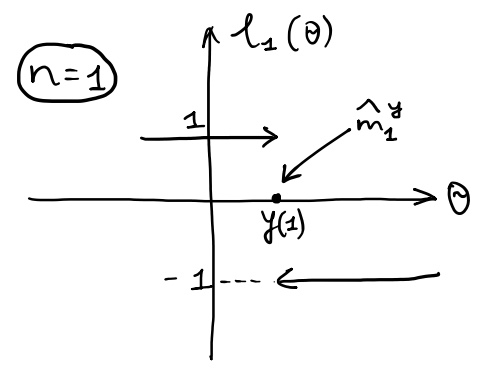
\includegraphics[width=90mm]{lec9im1}
			\columnbreak
			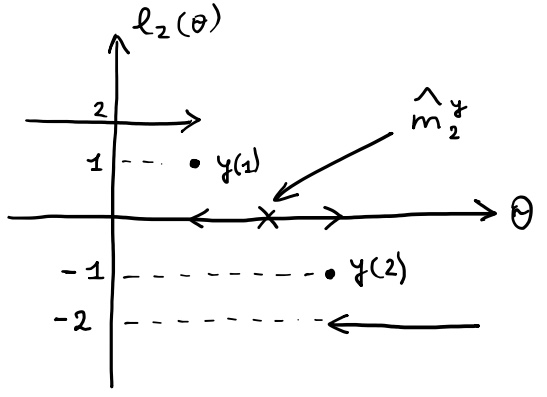
\includegraphics[width=90mm]{lec9im2}
		\end{multicols}
	\end{figure}

	Так бывает всегда: при нечетном $n$ решение уравнения (2) всегда существует и единственно - это $\hat{m}_n^y$; при четном $n$ решений целый интервал и $\hat{m}_n^y$ - его середина.

	В силу ЗБЧ при любом $\theta$ и любом $0 \le \gamma \le 1$:
	$$l_n (\theta) = n^{-1} \underset{t=1}{\overset{n}{\sum}}sign (y_t - \theta) \xrightarrow[n \to \infty]{P} E sign(y_1 - \theta) =: \Lambda_M (\gamma, \theta)$$

	\begin{problem} Пусть $\xi, \; \eta$ -- независимые случайные векторы, причем $\eta$ -- дискретный вектор со значениями $\eta_1, \eta_2, \ldots$. Необходимо проверить, что 
	$$E\varphi(\xi, \eta) = \sum\limits_{k \geq 1} E\varphi(\xi, \eta_k)P(\eta = \eta_k) = \sum\limits_{k \geq 1} E(\varphi(\xi, \eta) | H_k)P(H_k),$$ 
	где гипотеза $H_k = (\eta = \eta_k)$.
	\end{problem}

	Найдем удобный вид для $\Lambda_M(\gamma, \theta)$. Имеем
	$$\Lambda_M(\gamma, \theta) = E(1- 2 I(y_1 - \theta \leq 0)) = 1 - 2EI(\varepsilon_1 \leq \theta - a - z^{\gamma}_1 \xi_1) = 1 - 2EG(\theta - a - z^{\gamma}_1 \xi_1), \eqno(3)$$
	т.к. $sign(x) = 1 - 2I(x < 0)$ при $x \neq 0$.

	Чтобы упростить (3), введем две гипотезы: $H_1 = (z^{\gamma}_1 = 0), \; H_2 = (z^{\gamma}_2 = 1)$. Тогда, используя задачу, получим из (3), что $$\Lambda_M(\gamma, \theta) = 1 - 2(1 - \gamma)G(\theta - a) - 2\gamma EG(\theta - a - \xi_1).$$ Функция $\Lambda_M(\gamma, \theta)$ определена при всех $\gamma, \; \theta$, в том числе для отрицательных $\gamma$.

	\textit{ШАГ 2}.\\
	Функция $\Lambda_M(\gamma, \theta)$ в окрестности точки (0, a) удовлетворяет всем предположениям теоремы о неявной функции. А именно:

	\begin{enumerate}
		\item $\Lambda_M(0, a) = 1 - 2G(0) = 0;$
		\item Существуют и непрерывнф по паре $(\gamma, \theta)$ фнкции $\dfrac{\partial\Lambda_M(\gamma, \theta)}{\partial\gamma}, \; \dfrac{\partial\Lambda_M(\gamma, \theta)}{\partial\theta};$
		\item $\dfrac{\partial\Lambda_M(\gamma, \theta)}{\partial\theta} = -2g(0) \neq 0.$
	\end{enumerate}

	Значит, в окрестности точки (0, a) определена функция $\theta_m(\gamma) = \theta_{\gamma}^m$ такая, что $\Lambda_M(\gamma, \theta_{\gamma}^m) = 0.$ Кроме того, $\theta_{0}^m = a, \; \theta_{\gamma}^m \longrightarrow \theta_0$ при $\gamma \longrightarrow 0$. Функция $\theta_{\gamma}^m$ дифференцируема в точке $\gamma = 0$, и 
	$$\dfrac{d \theta_{\gamma}^m}{d\gamma} \mid_{\gamma = 0} = -(\dfrac{\partial \Lambda_M(0, a)}{\partial\theta})^{-1} \dfrac{\partial \Lambda_M(0, a)}{\partial\gamma} = \dfrac{1 - 2EG(-\xi_2)}{2g(0)} \eqno(4)$$

	\textit{ШАГ 3}.\\
	Покажем, что 
	$$\hat{m_n^y} \longrightarrow \theta_{\gamma}^m, \; n \longrightarrow \infty\eqno(5)$$
	Тогда из (4), (5) будет следовать, что функционал влияния  выборочной медианы равен 
	$$IF(\theta_{\gamma}^m, \mu_{\xi}) = \dfrac{1 - 2EG(-\xi_1)}{2g(0)}\eqno(6)$$
	Модуль числителя в (6) не больше 1, причем, если $\xi_1$ неслучайно и $\xi_1 \longrightarrow +\infty,$ то числитель стремится к 1. Значит, 
	$$GES(\theta_{\gamma}^m, M_{\xi}) = \underset{\mu_{\xi} \in M_{\xi}}{sup}|IF(\theta_{\gamma}^m, \mu_{\xi})| = \dfrac{1}{2g(0)}.$$
	Итак, докажем (5). Имеем при малых $\gamma$ ($\gamma$ фиксированно!) и $\theta$ вблизи a:
	$$\dfrac{\partial\Lambda_M(\gamma, \theta)}{\partial\theta} = -2(1 - \gamma)g(\theta - a) - 2\gamma Eg(\theta - a - \xi_1) < 0$$ 
	То есть $\Lambda(\gamma, \theta)$ убывает по $\theta.$ Значит,
	$$\begin{cases}
	\Lambda_M(\gamma, \theta_{\gamma}^m - \Delta) > 0 \\
	\Lambda_M(\gamma, \theta_{\gamma}^m + \Delta) < 0
	\end{cases},$$ но
	$$\begin{cases}
	l_n(\theta_{\gamma}^m - \Delta) \stackrel{P}{\longrightarrow} \Lambda_M(\gamma, \theta_{\gamma}^m - \Delta) > 0 \\
	l_n(\theta_{\gamma}^m + \Delta) \stackrel{P}{\longrightarrow} \Lambda_M(\gamma, \theta_{\gamma}^m + \Delta) < 0
	\end{cases} \eqno(7)$$
	Функция $l_n(\theta)$ монотонно убывает (точнее, не возрастет) по $\theta$. В силу (7) с вероятностью сколь угодно близкой к единице при достаточно больших n все корни уравнения $l_n(\theta) = 0$ лежат в интервале $(\theta_{\gamma}^m - \Delta, \theta_{\gamma}^m + \Delta)$. Выборочная медиана $\hat{m_n^y}$ тоже лежит в этом интервале! Поскольку $\Delta > 0$ любое, получаем, что 
	$$\hat{m_n^y} \stackrel{P}{\longrightarrow} \theta_{\gamma}^m, \; n \longrightarrow \infty.$$ 
\end{Proof}

\section{Нахождение функционала влияния в общем случае}\label{lec:9/sec:2}

Пусть оценка $\hat{\beta_n}$ ищется как корень уравнения
$$l_n(\theta) := n^{-1}\sum\limits_{t = 1}^n \varphi(\mathcal{I}_n, \theta) = 0 \eqno(1)$$
Пусть выполнены следующие условия:

 $$(i) l_n(\theta) = n^{-1}\sum\limits_{t = 1}^n \varphi(\mathcal{I}_n, \theta) \stackrel{P}{\longrightarrow} \Lambda(\gamma, \theta) \text{ при всех } |\theta - \beta| < \delta, \; 0 \geq \gamma < \gamma_0$$
 $$(ii) \Lambda(0, \beta) = 0$$
 $$\begin{gathered}(iii) \text{Пусть } \Lambda(\gamma, \theta) \text{ можно продолжить на отрицательные малые } \gamma \text{ так, что}\\ 
 \text{при }  |\theta - \beta| < \delta, \; |\gamma| < \gamma_0 \text{ существуют и непрерывны по паре } (\gamma, \theta) \text{ функции }\\ 
 \dfrac{\partial\Lambda(\gamma, \theta)}{\partial\gamma}, \; \dfrac{\partial\Lambda(\gamma, \theta)}{\partial\theta}\end{gathered}$$
 $$(iV)\text{Пусть } \lambda(\beta) := \dfrac{\partial\Lambda(\gamma, \theta)}{\partial\theta} \neq 0$$

\begin{theorem}\label{cha:12/the:2}
	Пусть выполнены условия (i)-(iV), функции $\varphi(\mathcal{I}_n, \theta)$ непрерывны по $\theta$. Тогда уравнение (1) с вероятностью, стремящейся к 1 при $n \longrightarrow \infty$, имеет при достаточно малых $\gamma \geq 0$ такое решение $\hat{\beta_n}$, что соответствующая оценка $\hat{\beta_n} \stackrel{P}{\longrightarrow} \theta_{\gamma}, \; \theta_0 = 0,$ и $\exists$ функционал влияния  
	$$IF(\theta_{\gamma}, \mu_{\xi}) = -(\lambda(\beta))^{-1} \dfrac{\partial}{\partial\gamma}\Lambda(0, \beta).$$
\end{theorem}

\section{М - оценка медианы}\label{lec:10/sec:1}

%\begin{center}
%\textit{\underline{М - оценка медианы.}}
%\end{center}\vspace{1cm}

Пусть 
$$
\begin{cases}
u_t = a + \varepsilon_t \\
y_t = u_t + z_t^g\xi_t, 
\end{cases}
$$

где $ \lbrace \varepsilon_t \rbrace $ -- н.о.р., $ \varepsilon_1 \sim g(x) = G'(x), \; g(x) = g(-x). $ Тогда $ a $ -- медиана ф.р. сл.в. $ u_1 .$ Будем искать оценку $ a $ (обозначим ее $ \hat{a_n} $) как корень уравнения 
$$\sum\limits_{t = 1}^n\psi(y_t - \theta) = 0\eqno(9)$$

Такая оценка называется \red{М - оценкой}. Вчастности, при $ \psi(x) = x, \; \hat{a_n} = \bar{y},  $ при $ \psi(x) = sign(x)\; \hat{a_n} = \hat{m_n}^y. $

Пусть выполнены условия:

\begin{enumerate}
\item $ \psi(x) $ -- нечетная строго возрастающая функция, $\underset{x \to +\infty}{\overset{}{\lim}} \psi(x) = c_1 > 0$, \\$\underset{x \to -\infty}{\overset{}{\lim}}\psi(x) = c_2 < \infty$
\item $ \exists $ непрерывная и ограниченная $ \psi'(x), \; E\psi'(\varepsilon_1) \neq 0 $
\end{enumerate}

Тогда уравнение (9) всегда имеет единственное решение. Условия 1, 2 выполнены, например, для $ \psi(x) = \arctan(x), \; \underset{x \to +\infty}{\overset{}{\lim}}\psi(x) = \dfrac{\pi}{2}, \;  \underset{x \to -\infty}{\overset{}{\lim}}\psi(x) = -\dfrac{\pi}{2}, \; \psi'(x) = \dfrac{1}{x^2 + 1}$.

Найдем функционал влияния и чувствительность М - оценки. Используем теорему \ref{cha:12/the:2}. Проверим условия: 
$$n^{-1}\sum\limits_{t = 1}^n \psi(y_t - \theta ) \stackrel{P}{\longrightarrow} E\psi(y_1 - \theta) =: \Lambda(\gamma, \theta) \text{ при всех } \theta, \; 0 \leq \gamma \leq 1\eqno(i)$$
Введем гипотезы $ H_1 = (z_1^\gamma = 0), \; H_2 = (z_2^\gamma = 1) .$
 Тогда: 
 $$ \begin{gathered}
 	\Lambda(\gamma, \theta) = \sum\limits_{i = 2}^n E(\psi(\underbrace{\varepsilon_1 + a + z_1^\gamma \xi_1}_{= y_1} - \theta) \mid H_i) \times P(H_i) = \\
 	= (1 - \gamma)E\psi(\varepsilon_1 + a - \theta) + \gamma E\psi(\varepsilon_1 + \xi_1 + a - \theta)
 \end{gathered}$$
 
$$ \Lambda(0, a) = E\psi(\varepsilon_1) = 0\eqno(ii)$$ 
т.к. $ \Lambda(\gamma, \theta) $ определена при всех $ \gamma $ и $ \theta . \; \dfrac{\partial \Lambda(\gamma, \theta)}{\partial \gamma}, \; \dfrac{\partial \Lambda(\gamma, \theta)}{\partial \theta} $ существуют при условиях (i), (ii) и непрерывна по паре $ (\gamma, \theta) $. В частности,  
$$
\begin{gathered}
\dfrac{\partial \Lambda(\gamma, \theta)}{\partial \gamma} = -E\psi(\varepsilon_1) + E\psi(\varepsilon_1 + \xi_1) = 0 + E\psi(\varepsilon_1 + \xi_1).
\end{gathered}
$$
 
$$ \dfrac{\partial \Lambda(0, a)}{\partial \theta} = -E\psi'(\varepsilon_1) \neq 0\eqno(iii)$$

В силу теоремы \ref{cha:12/the:2} $ \hat{a_n}  \stackrel{P}{\longrightarrow} \theta_\gamma, \; \theta_0 = a, $ 
$$
\begin{gathered}
IF(\theta_\gamma, \mu_\xi) = \dfrac{E\psi(\varepsilon_1 + \xi_1)}{E\psi'(\varepsilon_1)}, \\
GES(\theta_\gamma, M_\xi) \leq \dfrac{max(|c_1|, |c_2|)}{E\psi'(\varepsilon_1)} < \infty,
\end{gathered}
$$
$ M_\xi $ -- класс всех вер. распределений.